\documentclass[12pt,b5paper]{ltjsarticle}

%\usepackage[margin=15truemm, top=5truemm, bottom=5truemm]{geometry}
%\usepackage[margin=10truemm,left=15truemm]{geometry}
\usepackage[margin=10truemm]{geometry}

\usepackage{amsmath,amssymb}
%\pagestyle{headings}
\pagestyle{empty}

%\usepackage{listings,url}
%\renewcommand{\theenumi}{(\arabic{enumi})}

\usepackage{graphicx}

%\usepackage{tikz}
%\usetikzlibrary {arrows.meta}
%\usepackage{wrapfig}	% required for `\wrapfigure' (yatex added)
%\usepackage{bm}	% required for `\bm' (yatex added)

% ルビを振る
%\usepackage{luatexja-ruby}	% required for `\ruby'

%% 核Ker 像Im Hom を定義
%\newcommand{\Img}{\mathop{\mathrm{Im}}\nolimits}
%\newcommand{\Ker}{\mathop{\mathrm{Ker}}\nolimits}
%\newcommand{\Hom}{\mathop{\mathrm{Hom}}\nolimits}

%\DeclareMathOperator{\Rot}{rot}
%\DeclareMathOperator{\Div}{div}
%\DeclareMathOperator{\Grad}{grad}
%\DeclareMathOperator{\arcsinh}{arcsinh}
%\DeclareMathOperator{\arccosh}{arccosh}
%\DeclareMathOperator{\arctanh}{arctanh}



%\usepackage{listings,url}
%
%\lstset{
%%プログラム言語(複数の言語に対応,C,C++も可)
%  language = Python,
%%  language = Lisp,
%%  language = C,
%  %背景色と透過度
%  %backgroundcolor={\color[gray]{.90}},
%  %枠外に行った時の自動改行
%  breaklines = true,
%  %自動改行後のインデント量(デフォルトでは20[pt])
%  breakindent = 10pt,
%  %標準の書体
%%  basicstyle = \ttfamily\scriptsize,
%  basicstyle = \ttfamily,
%  %コメントの書体
%%  commentstyle = {\itshape \color[cmyk]{1,0.4,1,0}},
%  %関数名等の色の設定
%  classoffset = 0,
%  %キーワード(int, ifなど)の書体
%%  keywordstyle = {\bfseries \color[cmyk]{0,1,0,0}},
%  %表示する文字の書体
%  %stringstyle = {\ttfamily \color[rgb]{0,0,1}},
%  %枠 "t"は上に線を記載, "T"は上に二重線を記載
%  %他オプション:leftline,topline,bottomline,lines,single,shadowbox
%  frame = TBrl,
%  %frameまでの間隔(行番号とプログラムの間)
%  framesep = 5pt,
%  %行番号の位置
%  numbers = left,
%  %行番号の間隔
%  stepnumber = 1,
%  %行番号の書体
%%  numberstyle = \tiny,
%  %タブの大きさ
%  tabsize = 4,
%  %キャプションの場所("tb"ならば上下両方に記載)
%  captionpos = t
%}



\begin{document}

\hrulefill

次の積分を求めよ。
\begin{equation}
 \int_{0}^{\infty} \frac{\sqrt{x}}{x^3+1}\mathrm{d}x
\end{equation}

\dotfill

この広義積分を複素数上の積分として考える。
$R$は十分に大きい値をとり、$\varepsilon$は十分に$0$に近い値をとる。
\begin{equation}
  \int_{0}^{\infty} \frac{\sqrt{x}}{x^3+1}\mathrm{d}x
   =
   \lim_{\substack{R \to \infty \\ \varepsilon \to 0}}
   \int_{\varepsilon}^{R} \frac{\sqrt{z}}{z^3+1}\mathrm{d}z
  \qquad (z\in\mathbb{C})
\end{equation}

被積分関数$f(z)=\frac{\sqrt{z}}{z^3+1}$に対して、
積分経路を次のように考える。

複素平面上において、
$0$中心の半径$R$の円周と、
半径$\varepsilon$の円周、
$\varepsilon > \delta > 0$となる$\delta$を利用し
実数直線の正の部分を$+\delta i$だけ平行移動した直線と、
実数直線の正の部分を$-\delta i$だけ平行移動した直線
の4つを作る。
半径$\varepsilon$の円と$+\delta i$だけ平行移動した直線との交点を$P_1$、
半径$R$の円と$+\delta i$だけ平行移動した直線との交点を$P_2$、
半径$R$の円と$-\delta i$だけ平行移動した直線との交点を$P_3$、
半径$\varepsilon$の円と$-\delta i$だけ平行移動した直線との交点を$P_4$とする。

$P_1$から$P_2$へ向かう直線を$C_1$、
$P_2$から円周を反時計回りに回って$P_3$へ向かう曲線を$C_2$、
$P_3$から$P_4$へ向かう直線を$C_3$、
$P_4$から円周を時計回りに回って$P_1$へ向かう曲線を$C_4$とする。
この時の複素数$z$の偏角は$0$から$2\pi$の間の値をとるものとする。
($0 \leq \arg{z} \leq 2\pi$)

この4つの積分路をつないで一つの積分路とし、
$C$で表す。
($C=C_1+C_2+C_3+C_4$)


\begin{enumerate}
 \item [$C_1$]

       $P_1$から$P_2$へ向かう直線であり、
       この直線上の複素数は
       $z=x+\delta i \ (x\in\mathbb{R})$
       である。

 \item [$C_2$]

       $P_2$から円周を反時計回りに回って$P_3$へ向かう曲線であり、
       円周上の複素数は
       $z=Re^{i\theta} \ (\theta\in\mathbb{R},0\leq\theta\leq2\pi)$
       である。

 \item [$C_3$]

       $P_3$から$P_4$へ向かう直線であり、
       この直線上の複素数は
       $z=x-\delta i \ (x\in\mathbb{R})$
       である。

 \item [$C_4$]

       $P_4$から円周を時計回りに回って$P_1$へ向かう曲線であり、
       円周上の複素数は
       $z=\varepsilon e^{i\theta} \ (\theta\in\mathbb{R},0\leq\theta\leq2\pi)$
       である。

\end{enumerate}

%%%
%%% 図
%%%
\begin{figure}
\label{fig:hoge}
\centerline{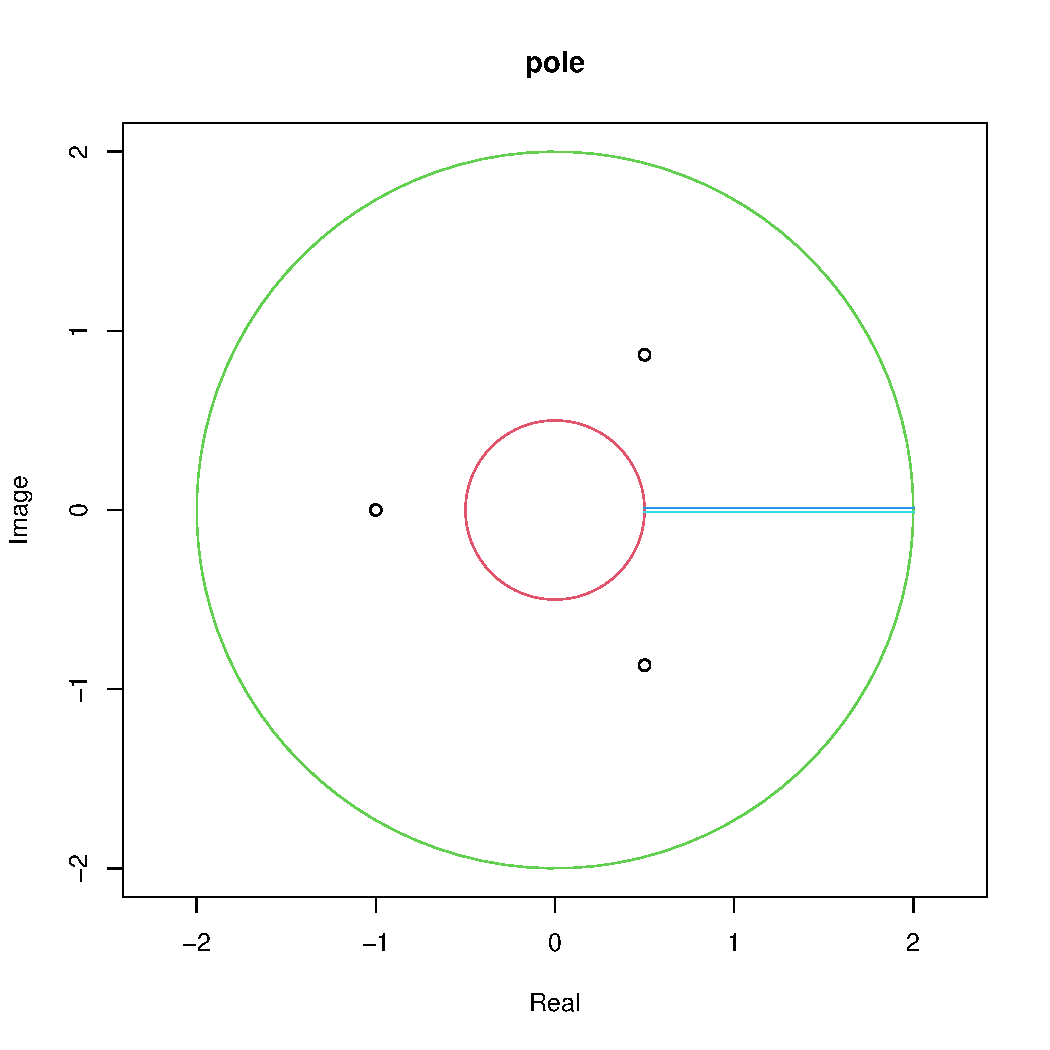
\includegraphics[width=0.5\textwidth]{pole_plot_R.pdf}}
\caption{極の場所と積分経路}
\end{figure}






$C$上の積分は次のような式となる。
\begin{equation}
 \int_{C} f(z)\mathrm{d}z
  =
 \int_{C_1} f(z)\mathrm{d}z
 +
 \int_{C_2} f(z)\mathrm{d}z
 +
 \int_{C_3} f(z)\mathrm{d}z
 +
 \int_{C_4} f(z)\mathrm{d}z
\end{equation}


$\delta \to 0$と極限をとれば
各積分路上の複素数$z$は次のような式で表される。
\begin{enumerate}
 \item [$C_1$]

       $z=x e^{0i} \ (x:\varepsilon \to R)$

 \item [$C_2$]

       $z=Re^{i\theta} \ (\theta : 0\to 2\pi)$

 \item [$C_3$]

       $z=x e^{2\pi i} \ (x:R\to\varepsilon)$

 \item [$C_4$]

       $z=\varepsilon e^{i\theta} \ (\theta : 2\pi \to 0)$

\end{enumerate}

%%%
%%% 図
%%%

積分路$C$は閉じているので、
留数定理により
積分$\int_{C}f(z)\mathrm{d}z$は
$C$の内部にある極から求まる。

$f(z)=\frac{\sqrt{z}}{z^3+1}$の極は
$z^3+1=0$を満たし、
$R$が十分に大きく$\varepsilon$が十分に小さいので
全て$C$の内部に存在する。

$z^3+1=0$を満たす複素数は
$z^3=-1=e^{(2n+1)\pi i}$から
$z=e^{\frac{\pi}{3}i},e^{\pi i},e^{\frac{5\pi}{3}i}$
である。
つまり次のような因数分解ができる。
$z^3+1 = (z-e^{\frac{\pi}{3}i})(z-e^{\pi i})(z-e^{\frac{5\pi}{3}i})$

留数定理により
$\int_{C} f(z)\mathrm{d}z$
は
3つの極$z=e^{\frac{\pi}{3}i},e^{\pi i},e^{\frac{5\pi}{3}i}$
それぞれのの留数から求まる。

オイラーの公式により極は次の複素数と等しい。
\begin{align}
 e^{\frac{\pi}{3}i} =& \cos{\frac{\pi}{3}}+i\sin{\frac{\pi}{3}}
  = \frac{1}{2}+\frac{\sqrt{3}}{2}i\\
 e^{\pi i} =& \cos{\pi}+i\sin{\pi}
  = -1\\
 e^{\frac{5\pi}{3}i} =& \cos{\frac{5\pi}{3}}+i\sin{\frac{5\pi}{3}}
  = \frac{1}{2}-\frac{\sqrt{3}}{2}i
\end{align}

これらを用いて3つの極の留数を求める。
\begin{align}
 \mathrm{Res}(f,e^{\frac{\pi}{3}i})
  =&
 \lim_{z\to e^{\frac{\pi}{3}i}}(z-e^{\frac{\pi}{3}i})\times \frac{\sqrt{z}}{z^3+1}
  =
 \lim_{z\to e^{\frac{\pi}{3}i}} \frac{\sqrt{z}}{(z-e^{\pi i})(z-e^{\frac{5\pi}{3}i})}\\
 =&
 \frac{\sqrt{e^{\frac{\pi}{3}i}}}{(e^{\frac{\pi}{3}i}-e^{\pi i})(e^{\frac{\pi}{3}i}-e^{\frac{5\pi}{3}i})}
 =
 \frac{e^{\frac{\pi}{6}i}}{(\frac{3}{2}+\frac{\sqrt{3}}{2}i)\times \sqrt{3}i}\\
 =& \frac{e^{\frac{\pi}{6}i}}{3(\frac{\sqrt{3}}{2}i-\frac{1}{2})}
 = \frac{e^{\frac{\pi}{6}i}}{3 e^{\frac{2\pi}{3}i}}
 = \frac{e^{-\frac{\pi}{2}i}}{3}
 = -\frac{1}{3}i
 \\
 %
 \mathrm{Res}(f,e^{\pi i})
 =&
 \lim_{z\to e^{\pi i}}(z-e^{\pi i})\times \frac{\sqrt{z}}{z^3+1}
 =
 \lim_{z\to e^{\pi i}} \frac{\sqrt{z}}{(z-e^{\frac{\pi}{3}i})(z-e^{\frac{5\pi}{3}i})}\\
 =&
 \frac{\sqrt{e^{\pi i}}}{(e^{\pi i}-e^{\frac{\pi}{3}i})(e^{\pi i}-e^{\frac{5\pi}{3}i})}
 =
 \frac{e^{\frac{\pi}{2} i}}{(e^{\pi i}-e^{\frac{\pi}{3}i})(e^{\pi i}-e^{\frac{5\pi}{3}i})}
 \\
 =&
 \frac{e^{\frac{\pi}{2} i}}{e^{\pi i}e^{\pi i}-e^{\frac{\pi}{3}i}e^{\pi i}-e^{\pi i}e^{\frac{5\pi}{3}i}+e^{\frac{\pi}{3}i}e^{\frac{5\pi}{3}i}}\\
 =&
 \frac{e^{\frac{\pi}{2} i}}{1-e^{\frac{4\pi}{3}i}-e^{\frac{8\pi}{3}i}+1}
 =
 \frac{e^{\frac{\pi}{2} i}}{2-(-\frac{1}{2}-\frac{\sqrt{3}}{2}i) - (-\frac{1}{2}+\frac{\sqrt{3}}{2}i)}
 =
 \frac{1}{3}i\\
 %
 \mathrm{Res}(f,e^{\frac{5\pi}{3}i})
 =&
 \lim_{z\to e^{\frac{5\pi}{3}i}}(z-e^{\frac{5\pi}{3}i})\times \frac{\sqrt{z}}{z^3+1}
 =
 \lim_{z\to e^{\frac{5\pi}{3}i}} \frac{\sqrt{z}}{(z-e^{\frac{\pi}{3}i})(z-e^{\pi i})}\\
=&
 \frac{\sqrt{e^{\frac{5\pi}{3}i}}}{(e^{\frac{5\pi}{3}i}-e^{\frac{\pi}{3} i})(e^{\frac{5\pi}{3}i}-e^{\pi i})}
 =
 \frac{e^{\frac{5\pi}{6}i}}{-\sqrt{3}i(\frac{3}{2}-\frac{\sqrt{3}}{2}i)}\\
 =&
 \frac{e^{\frac{5\pi}{6}i}}{3(-\frac{\sqrt{3}}{2}i-\frac{1}{2})}
 =
 \frac{e^{\frac{5\pi}{6}i}}{3e^{\frac{4\pi}{3}i}}
 =
 \frac{e^{-\frac{\pi}{2}i}}{3}
 =
 - \frac{1}{3}i
\end{align}


これにより、$C$上の積分は次のようになる。
\begin{equation}
 \int_{C} \frac{\sqrt{z}}{z^3+1}\mathrm{d}z
  = 2\pi i \left(-\frac{1}{3}i +  \frac{1}{3}i - \frac{1}{3}i \right)
  =  \frac{2\pi}{3}
\end{equation}


$C$は4つに分かれるためそれぞれの積分を考える。

$C_1$は直線であり、
$z=x e^{0i}=x \ (x:\varepsilon \to R)$
となる複素数での積分である。
この時$\mathrm{d}z=\mathrm{d}x$である。
\begin{equation}
 \int_{C_1} f(z)\mathrm{d}z
  =\int_{\varepsilon}^{R} \frac{\sqrt{x}}{x^3+1}\mathrm{d}x
  \to \int_{0}^{\infty} \frac{\sqrt{x}}{x^3+1} \mathrm{d}x \ (\varepsilon\to 0, R\to\infty)
\end{equation}

$C_2$は半径$R$の円周上であり、
$z=Re^{i\theta} \ (\theta : 0\to 2\pi)$となる複素数での積分である。
このとき、$\mathrm{d}z = iRe^{i\theta}\mathrm{d}\theta$である。
\begin{align}
 \int_{C_2} f(z)\mathrm{d}z
 = \int_{0}^{2\pi} \frac{\sqrt{Re^{i\theta}}}{(Re^{i\theta})^3+1} iRe^{i\theta}\mathrm{d}\theta
 = \int_{0}^{2\pi} \frac{iR^{\frac{3}{2}}e^{\frac{3}{2}i\theta}}{R^3 e^{3i\theta}+1} \mathrm{d}\theta
\end{align}


\begin{align}
  \left\lvert \int_{0}^{2\pi} \frac{iR^{\frac{3}{2}}e^{\frac{3}{2}i\theta}}{R^3 e^{3i\theta}+1} \mathrm{d}\theta \right\rvert
  \leq &
   \int_{0}^{2\pi} \left\lvert \frac{iR^{\frac{3}{2}}e^{\frac{3}{2}i\theta}}{R^3 e^{3i\theta}+1}  \right\rvert \mathrm{d}\theta\\
   = &
   \int_{0}^{2\pi}  \frac{\lvert iR^{\frac{3}{2}}e^{\frac{3}{2}i\theta} \rvert}{\lvert R^3 e^{3i\theta}+1 \rvert}   \mathrm{d}\theta
   =
   \int_{0}^{2\pi}
   \frac{\lvert i \rvert \lvert R^{\frac{3}{2}}\rvert \lvert e^{\frac{3}{2}i\theta} \rvert}
   {\lvert e^{3i\theta} \rvert \lvert R^3 + e^{-3i\theta} \rvert}
   \mathrm{d}\theta
\end{align}

$\theta\in\mathbb{R}$について
$\lvert e^{-3i\theta} \rvert = \lvert e^{\frac{3}{2}i\theta} \rvert =\lvert i \rvert= 1$
となる。
$R$が十分に大きい値であれば
$\lvert R^3 + e^{-3i\theta} \rvert \geq  R^3 -1$
であるので、これを利用し上の式を計算する。
\begin{equation}
   \int_{0}^{2\pi}
   \frac{\lvert i \rvert \lvert R^{\frac{3}{2}}\rvert \lvert e^{\frac{3}{2}i\theta} \rvert}
   {\lvert e^{3i\theta} \rvert \lvert R^3 + e^{-3i\theta} \rvert}
   \mathrm{d}\theta
   \leq
  \int_{0}^{2\pi}\frac{R^{\frac{3}{2}}}{R^3-1}\mathrm{d}\theta
  = \frac{R^{\frac{3}{2}}}{R^3-1}\cdot2\pi
  \to 0 \ (R\to\infty)
\end{equation}

つまり、$C_2$上の積分は$R\to\infty$において$0$に収束する。
\begin{equation}
 \lim_{R\to\infty}\int_{C_2} f(z)\mathrm{d}z=0
\end{equation}

次に$C_3$上の積分を考える。
$C_3$は直線であり、
$z=x e^{2\pi i} \ (x:R\to\varepsilon)$
となる複素数での積分である。
この時$\mathrm{d}z=e^{2\pi i}\mathrm{d}x$である。

\begin{align}
  \int_{C_3} f(z)\mathrm{d}z
   =
  \int_{R}^{\varepsilon} \frac{\sqrt{x e^{2\pi i}}}{(x e^{2\pi i})^3+1}e^{2\pi i}\mathrm{d}x
  =
  \int_{R}^{\varepsilon} \frac{x^{\frac{1}{2}} e^{\pi i}}{x^3 e^{6\pi i}+1}e^{2\pi i}\mathrm{d}x\\
  =\int_{R}^{\varepsilon} \frac{-x^{\frac{1}{2}}}{x^3 +1}\mathrm{d}x
  =\int_{\varepsilon}^{R} \frac{x^{\frac{1}{2}}}{x^3 +1}\mathrm{d}x
 \to \int_{0}^{\infty} \frac{\sqrt{x}}{x^3 +1}\mathrm{d}x \ (\varepsilon\to 0, R\to\infty)
\end{align}

よって、$C_3$上の積分は$C_1$上の積分と同じになる。

$C_4$上の積分を考える。
$C_4$は半径$\varepsilon$の円周上であり、
$z=\varepsilon e^{i\theta} \ (\theta : 2\pi \to 0)$となる複素数での積分である。
このとき、$\mathrm{d}z = i \varepsilon e^{i\theta}\mathrm{d}\theta$である。

\begin{equation}
 \int_{C_4}f(z)\mathrm{d}z
  = \int_{2\pi}^{0} \frac{\sqrt{\varepsilon e^{i\theta}}}{(\varepsilon e^{i\theta})^3+1} i\varepsilon e^{i\theta}\mathrm{d}\theta
  = \int_{2\pi}^{0} \frac{i\varepsilon^{\frac{3}{2}}e^{\frac{3}{2}i\theta}}{\varepsilon^3 e^{3i\theta}+1} \mathrm{d}\theta
\end{equation}

\begin{align}
 \left\lvert \int_{2\pi}^{0} \frac{i\varepsilon^{\frac{3}{2}}e^{\frac{3}{2}i\theta}}{\varepsilon^3 e^{3i\theta}+1} \mathrm{d}\theta \right\rvert
  =&
  \left\lvert \int_{0}^{2\pi} \frac{i\varepsilon^{\frac{3}{2}}e^{\frac{3}{2}i\theta}}{\varepsilon^3 e^{3i\theta}+1} \mathrm{d}\theta \right\rvert\\
  \leq &
  \int_{0}^{2\pi} \left\lvert \frac{i\varepsilon^{\frac{3}{2}}e^{\frac{3}{2}i\theta}}{\varepsilon^3 e^{3i\theta}+1} \right\rvert \mathrm{d}\theta
  =
  \int_{0}^{2\pi} \frac{\lvert i \rvert \lvert \varepsilon^{\frac{3}{2}}\rvert \lvert e^{\frac{3}{2}i\theta}\rvert}{\lvert e^{3i\theta}\rvert \lvert \varepsilon^3  + e^{-3i\theta} \rvert} \mathrm{d}\theta
\end{align}

ここで、
$\lvert e^{-3i\theta}\rvert =1$
となるので、
$\lvert \varepsilon^3  + e^{-3i\theta} \rvert \geq \lvert \varepsilon^3-1 \rvert $
であり、
十分に小さな$\varepsilon>0$において
$\lvert \varepsilon^3-1 \rvert =1-\varepsilon^3$
となる。
\begin{equation}
 \int_{0}^{2\pi} \frac{\lvert i \rvert \lvert \varepsilon^{\frac{3}{2}}\rvert \lvert e^{\frac{3}{2}i\theta}\rvert}{\lvert e^{3i\theta}\rvert \lvert \varepsilon^3  + e^{-3i\theta} \rvert} \mathrm{d}\theta
  \leq
  \int_{0}^{2\pi} \frac{\varepsilon^{\frac{3}{2}}}{1- \varepsilon^3} \mathrm{d}\theta
  =\frac{\varepsilon^{\frac{3}{2}}}{1- \varepsilon^3}\cdot 2\pi \to 0 \ (\varepsilon\to0)
\end{equation}

よって、$C_4$上の積分は$\varepsilon\to0$において
$0$に収束する。
\begin{equation}
 \lim_{\varepsilon\to 0}\int_{C_4}f(z)\mathrm{d}z=0
\end{equation}


\begin{equation}
 \int_{C} f(z)\mathrm{d}z
  =
 \int_{C_1} f(z)\mathrm{d}z
 +
 \int_{C_2} f(z)\mathrm{d}z
 +
 \int_{C_3} f(z)\mathrm{d}z
 +
 \int_{C_4} f(z)\mathrm{d}z
\end{equation}
であるが、
留数定理より
$\int_{C} f(z)\mathrm{d}z = \frac{2\pi}{3}$
である。

よって、次の式が成り立つ。
\begin{equation}
 \int_{C_1} f(z)\mathrm{d}z
 +
 \int_{C_2} f(z)\mathrm{d}z
 +
 \int_{C_3} f(z)\mathrm{d}z
 +
 \int_{C_4} f(z)\mathrm{d}z
 = \frac{2\pi}{3}
\end{equation}

これを移項し絶対値をとると
次の不等式が得られる。
\begin{align}
 \left\lvert
 \int_{C_1} f(z)\mathrm{d}z
 +
 \int_{C_3} f(z)\mathrm{d}z
 - \frac{2\pi}{3}
 \right\rvert
 = &
  \left\lvert
  \int_{C_2} f(z)\mathrm{d}z
  +
  \int_{C_4} f(z)\mathrm{d}z
 \right\rvert\\
  \leq &
  \left\lvert
  \int_{C_2} f(z)\mathrm{d}z
   \right\rvert
  +  \left\lvert
  \int_{C_4} f(z)\mathrm{d}z
 \right\rvert
\end{align}

不等式の右辺は
\begin{equation}
 \lim_{R\to\infty}\int_{C_2} f(z)\mathrm{d}z=
 \lim_{\varepsilon\to 0}\int_{C_4}f(z)\mathrm{d}z=0
\end{equation}
より、$0$に収束する。
これにより左辺も$0$に収束する。
また、$R\to\infty,\varepsilon\to 0$において
\begin{equation}
 \lim_{\substack{R \to \infty \\ \varepsilon \to 0}}\int_{C_1} f(z)\mathrm{d}z
  =
 \lim_{\substack{R \to \infty \\ \varepsilon \to 0}}\int_{C_3} f(z)\mathrm{d}z
 =
 \int_{0}^{\infty} \frac{\sqrt{x}}{x^3+1}\mathrm{d}x
\end{equation}
であるので、
\begin{equation}
  \int_{C_1} f(z)\mathrm{d}z
 +
 \int_{C_3} f(z)\mathrm{d}z
 - \frac{2\pi}{3}
\to
2\int_{0}^{\infty} \frac{\sqrt{x}}{x^3+1}\mathrm{d}x
 - \frac{2\pi}{3}
\ (R \to \infty ,\ \varepsilon \to 0)
\end{equation}

$2\int_{0}^{\infty} \frac{\sqrt{x}}{x^3+1}\mathrm{d}x
 - \frac{2\pi}{3}
=0$
より
\begin{equation}
 \int_{0}^{\infty} \frac{\sqrt{x}}{x^3+1}\mathrm{d}x
=\frac{\pi}{3}
\end{equation}
である。

\hrulefill

\end{document}
